\documentclass[12pt]{article}

\usepackage{verbatim} % For comments
\usepackage{setspace} % For double spacing
\usepackage{cite}  % For citations
\usepackage{url} % For url in citations...maybe
\usepackage{tabularx}
\usepackage{graphicx} % For graphics
\usepackage{multicol}

\doublespacing
\begin{document}

\title{A Replicable and Extensible Comparison of QUIC and TCP}
\author{Henry Baxter and Liam Simmons\\
		University of Victoria}
\date{\today}

\maketitle

	%Just wrote this abstract without any real references. Will proof/ rewrite after other sections are written.
\begin{abstract}
	Quick UDP Internet Connections (QUIC) is a transport protocol, first implemented by Google in 2013. Since then, it has seen rapid development over many version numbers. By design, QUIC is opaque to outside analysis. QUIC is encrypted, and exists in application space, to prevent ossification of the protocol, unlike TCP. Therefore, black-box analysis is required to study the performance of QUIC. We set out to compare the performance of QUIC and TCP. Further, we evaluate the protocols in a replicable and extensible way, to allow ease of future comparisons of the protocols. 
\end{abstract}

\section{Introduction}
\label{introduction}

QUIC (Quick UDP Internet Connections) is a new transport protocol, first implemented by Google in 2013. QUIC is designed to be optimized for HTTP traffic; it has several features that are similar to TCP+TLS, but is built on top of UDP. One major difference between TCP and QUIC is that QUIC is implemented in the userspace\cite{quicLayout}, whereas TCP exists within the OS kernel. While changes to TCP can take years to see wide-spread deployment, since QUIC exists as a self-contained protocol, QUIC sees rapid development. Further, QUIC is an encrypted protocol. This prevents QUIC from being tampered with by middleboxes and legacy systems, extending QUIC's ability to be quickly developed. 
% Citation for backwards incompatible changes every 6 weeks?

While these features allow QUIC to see swift development, they in turn make analysis of the protocol very difficult. Following the work of Kakhki, et al.\cite{Kakhki:2017:TLL:3131365.3131368}, we firstly replicate the work of Kakhki and verify their conclusions. We additionally modify their methodology to allow for replicability and tracking of future QUIC versions.

Comparison of QUIC and TCP is done in three testing environments. One, a local client makes requests to an EC2 instance that acts as the QUIC and TCP server, with an additional EC2 instance used to shape network traffic. The second testing environment exists entirely on an Amazon VLAN; one EC2 instance acts as a desktop computer, with two other EC2 instances acting as a router and server, as above. The third testing environment is similar to the second, with the exception that the EC2 Desktop is at a different physical location than the router and server. Parallel requests are made to the QUIC and TCP server, with variations in pages requested, as well as varying network conditions.

Our results show that QUIC outperforms TCP for nearly all variables tested from the local client. The one case where TCP outperforms QUIC from the local client is for very large numbers of objects. This finding is consistent with Kakhi, et al. For testing done within the Amazon VLAN, TCP slightly outperforms QUIC. This may suggest optimizations for TCP within AWS.

Our results suggest that QUIC is best for a consumer in most situations.
% More conclusions....

In section \ref{background}, we give a brief overview of the QUIC protocol, and the features that allow for improved performance over TCP. We also present related work on the analysis of QUIC. In \ref{methods}, our testbed and methodology are described in detail. In \ref{data}, the aggregation of our data is presented, and is discussed in \ref{results}. The conclusions of our findings are presented in \ref{conclusions}.

\section{Background}
\label{background}

\subsection{What is QUIC?}
\label{background:quic}

QUIC is a new transport protocol, first implemented by Google in 2013. Far from being an experimental protocol, QUIC is supported by all Google services, including the Chrome browser, YouTube app, and Google Search app on Android\cite{Langley:2017:QTP:3098822.3098842}. By Google's own estimation, in 2017 QUIC made up 7\% of Internet traffic\cite{Langley:2017:QTP:3098822.3098842}.

\begin{figure}
\centering
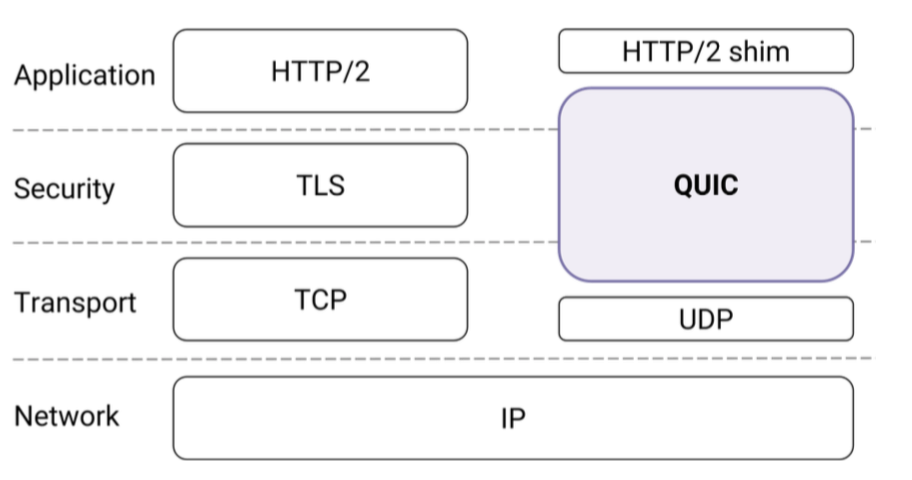
\includegraphics[scale=.25]{images/quic_stack.png}
\caption{QUIC in the traditional HTTPS stack. Image credit \cite{Langley:2017:QTP:3098822.3098842}}
\label{fig:quic_stack}
\end{figure}

QUIC is designed to optimize HTTPS traffic. It is functionally equivalent to TCP+TLS+HTTP/2\footnote{For the purpose of this report, \emph{TCP} will refer to \emph{TCP+TLS+HTTP/2}}, but is built on top of UDP. QUIC exists entirely within the userspace, which allows rapid evolution of the protocol. QUIC has several features that allow it to perform better than TCP, including:
\begin{itemize}
	\item \textbf{Reduced latency for connection establishment}
	\item \textbf{Stream multiplexing without head-of-line blocking}
	\item \textbf{Improved congestion control and loss recovery}
\end{itemize}

\textbf{Reduced Connection Latency:} QUIC combines both the transport and cryptographic handshake to reduce connection latency. For new connections, QUIC requires only 1-RTT to establish a connection\footnote{When there is no version negotiation}. This is one and two RTTs faster than TCP+TLS1.3 and TCP+TLS1.2, respectively\cite{7867726}. When a connection has been previously established, QUIC requires 0-RTT to re-establish the connection, by caching cryptographic values of the server on the client side.

\begin{figure}
\centering
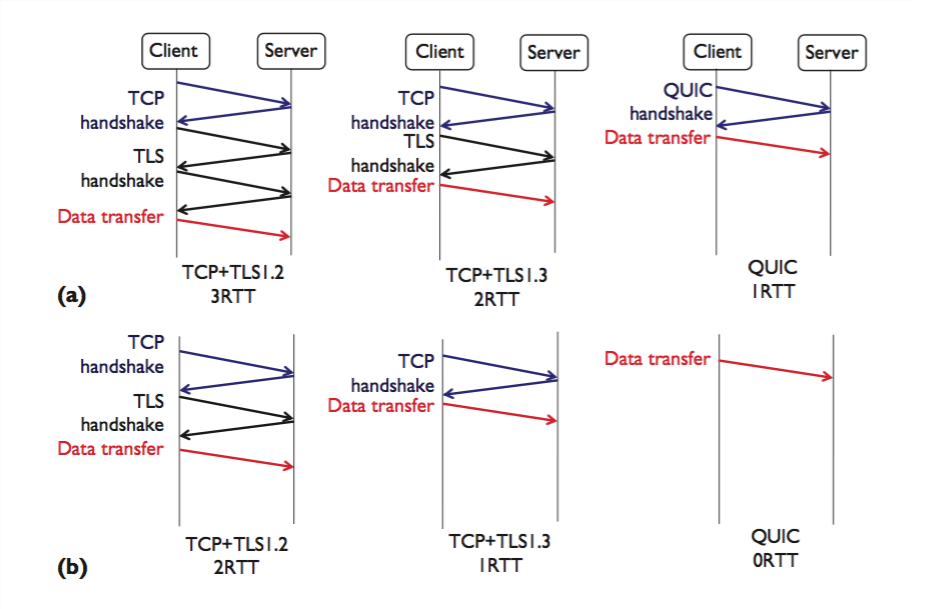
\includegraphics[scale=.3]{images/QUIC_TCP_RTT.png}
\caption{Handshake RTT of different protocols for (a) first time connection establishment and (b) subsequent connections. Image credit \cite{7867726}}
\label{fig:RTT}
\end{figure}

\textbf{Stream Multiplexing:} QUIC is designed for multiplexed operation; it allows multiple streams to exist for each connection. Within a QUIC stream, lost packets generally only affect that stream. Other streams can continue to make progress. QUIC can also abandon streams without concern. While HTTP/2 also features stream multiplexing, it exists on top of TCP's single byte-stream abstraction. When a segment is lost, all further segments are blocked until a retransmission occurs. QUIC reduces latency of retransmission by avoiding head-of-line blocking\cite{quicLayout}.

\begin{figure}
\centering
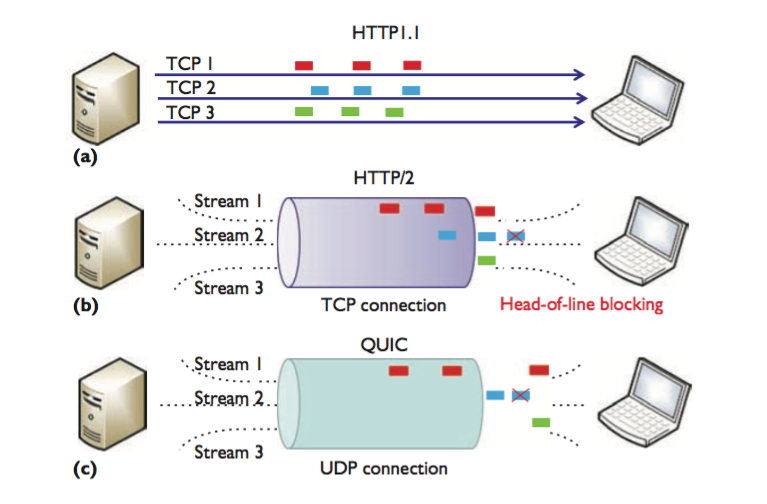
\includegraphics[scale=.4]{images/QUICmulti.png}
\caption{Multiplexing comparison of (a) HTTP1.1 (b) HTTP/2 and (c) QUIC. Image credit \cite{7867726}}
\label{fig:multiplex}
\end{figure}

\textbf{Improved Congestion Control and Loss Recovery:} For all packets, QUIC uses unique, monotonic sequence numbers. This allows QUIC to easily differentiate original from retransmitted packets, thus avoiding retransmission ambiguity found with TCP. QUIC ACK packets also explicitly carry the delay of packet reception to acknowledgment being sent, which allows QUIC to more accurately calculate RTT, and therefore further refine congestion control\cite{quicLayout}.

\subsection{Related Work}
\label{background:related}
As stated above, Kakhki et al. provides a starting point for our analysis. To the best of our knowledge, it is the most comprehensive comparison of QUIC and TCP to date. Further papers that provide analysis of QUIC performance include:

\begin{itemize}
	\item How Quick is QUIC?\cite{Megysei:2016:HQQ}
	\item HTTP over UDP: An Experimental Investigation of QUIC\cite{Carlucci:2015:HOU}
	\item Does QUIC make the web faster?\cite{Biswal:2016:DQM}
	\item Evaluation of QUIC in Web Page Performance\cite{Das:2014:EQW}
\end{itemize}

\section{Motivation}
\label{motivation}
QUIC is a rapidly evolving protocol, that is used for all Google services. As public analysis of QUIC is extremely limited as compared to TCP, it is vitally important that a deeper understanding of QUIC performance characteristics be both publicly accessible and replicable. With an experimental design focused on replicability and extensibility, we aim to provide both a comparative analysis of QUIC and TCP, as well as a model for future comparisons. In this way, future changes to the QUIC protocol can be quickly and efficiently tracked and analyzed.

\section{Methods}
\label{methods}
We now describe the methods used to compare the TCP and QUIC protocols.

% Which processor on local desktop? Which NGINX version? Is QUIC source accurate as described?
\subsection{Testbed}
Evaluation was performed in three different network environments, as shown in figure \ref{fig:network}.

The server and remote desktops run on Amazon EC2 T2.Large (Kernel 4.4.0-1054-aws, Ubuntu 16.04, 8 GB memory, Intel Xeon 3.0GHz\footnote{The T2 EC2 instance uses `burstable' CPU, so clock speed is \emph{up to} 3.0 GHz}).The router runs on Amazon EC2 T2.micro (Kernel 4.4.0-1054-aws, Ubuntu 16.04, 1 GB memory, Intel Xeon 3.3 GHz\footnote{Again, \emph{up to} 3.3 GHz}). The EC2 router and server are located on ec2-east1. One EC2 desktop is on ec2-east1 (as in fig. \ref{fig:network} (b)), and another on ec2-west1 (as in fig. \ref{fig:network} (c)).

The local client is a desktop (macOS High Sierra 10.13.4, 32 GB memory, Intel 2.4 GHz).

All clients run Google Chrome (ver. 65.0.3325.181 (Official Build) (64-bit)). The server supports HTTP/2 over TCP via NGINX 2.4, and over QUIC via the QUIC standalone server, as provided with the Chromium source code.

\begin{figure}
\begin{tabular}{c c}
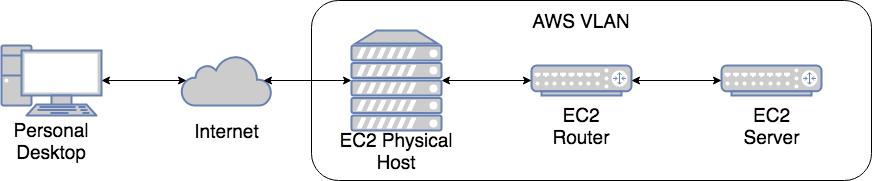
\includegraphics[scale=.25]{images/local.png} & 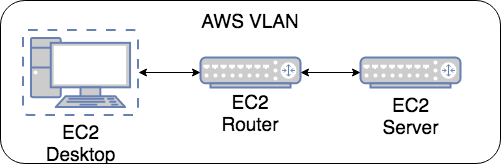
\includegraphics[scale=.25]{images/aws.png}\\
~ & ~ \\
(a) & (b) \\
~ & ~ \\
\multicolumn{2}{c}{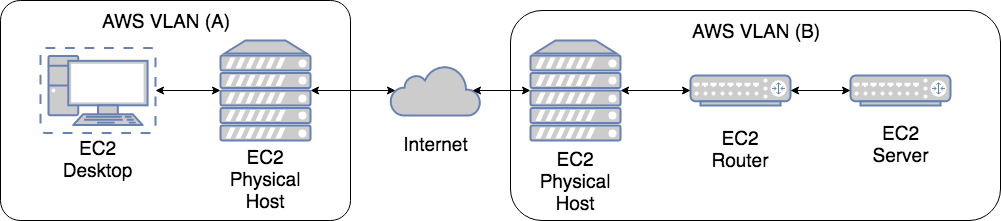
\includegraphics[scale=.25]{images/aws_inet.png}} \\
~ & ~ \\
\multicolumn{2}{c}{(c)} \\
\end{tabular}
\caption{Testbed setup for local (a), EC2 on same VLAN (b) and EC2 on separate VLAN (c)}
\label{fig:network}
\end{figure}

\subsection{Testing Variables}
Various treatments of network conditions were evaluated for each of the protocols. Parallel instances of Chrome were launched on either a local machine, or an EC2 instance. Treatments were generated from a configuration file, the variations are shown in table \ref{test_variables}. When a treatment is run, the test environment is automatically configured. Requests are initiated programmatically and page load time is captured for multiple runs. For each treatment, 100 iterations are performed of each protocol.

Network shaping was performed at the EC2 router using tc htb and qdisc.
% Going off of config file as of 04/11/18:46...update if there are others missing
\begin{figure}
\centering
\begin{tabular}{c|c}
	Parameter	&	Values tested 	\\\hline
	Object Size (KB)	&	5, 10, 100, 200, 500, 1000	\\
	Object Count &	5, 10, 50, 100, 500	\\
	Rate Limit (Mbps) 	&	5, 10, 25, 50	\\
	Packet Loss (\%)	&	0.0, 0.1, 1.0, 2.0	\\
	Latency (ms)		&	0, 50, 100, 200	\\
\end{tabular}
\caption{Test Variables}
\label{test_variables}
\end{figure}


\section{Data}
\label{data}

\section{Results}
\label{results}

\section{Conclusions}
\label{conclusions}

\appendix

\section{Contributions}
The following is a summary of the contributions of each team member:

\begin{tabularx}{\textwidth}{X|X}
Henry:	&	Liam:	\\ \hline
\textbullet Wrote the project proposal	&	\textbullet Set up website	\\
\textbullet Website Updates				&	\textbullet Website Updates	\\
\textbullet	Set up of QUIC, TCP Servers	&	\textbullet	Image creation for testing	\\
\textbullet	Writing of Python code for programmatic testing	&	\textbullet	Writing of Python code for page generation \\
\textbullet Running of tests			&	\textbullet Poster creation, outline \\
\textbullet Poster content 				&	\textbullet Poster content \\
\textbullet Overall data collection		&	\textbullet	Report outline \\
\textbullet	Report content 				&	\textbullet Report content \\
\end{tabularx}

\bibliography{bibliography}{}
\bibliographystyle{unsrt}
\end{document}